\section{Conceptual Design}

\subsection{Requirements}

	Objective of the database is to store the timetable of public transportation service within a single region. Following is a description of the information that is relevant and as such is represented in the database. \medskip
	
	A \textbf{trip} (identified by a code) consist of an ordered sequence of \textbf{stops}, each with arrival and departure times. The first stop of a trip does not have an arrival time, and the last one does not have a departure time. It \textbf{runs} on a defined period of the year, normally on specific days of the week and optionally on other dates, in which it can be exceptional or suppressed. \textit{For example, a trip could run within 14/09/2020 (included) and 26/06/2021 (excluded) from Monday to Friday, but not if the day is a public holiday. Another could run in the same dates range on Sunday, and also if the day is a public holiday.}
	
	A trip is part of a \textbf{line} and is conducted by a driver of a specific \textbf{company}, of which the name and the headquarter city are of interest. Of a line, the short code \textit{(e.g. 10A)}, a brief description \textit{(e.g. Hospital-City Centre-Hospital)}, the color, the city in which it originates and the type of vehicle \textit{(e.g. bus or train)} are of interest. The short code is unique only within a single city.
	
	A stop is instead characterized by the name, the \textbf{city} and the coordinates. When considering bus or train stations, the stopping point should also contain the platform name. The stop name should be memorized in different languages \textit{(e.g. in Italian and German)}. It is also the case that at least one translation is present, and if there is more than one translation, then all stop names are translated in all the possible languages.

\subsection{ER Schema}

	See Figure \ref{img:diagram} on next page.	

	\begin{landscape}
		\begin{figure}[htb]
			\thispagestyle{plain}
			\centering
			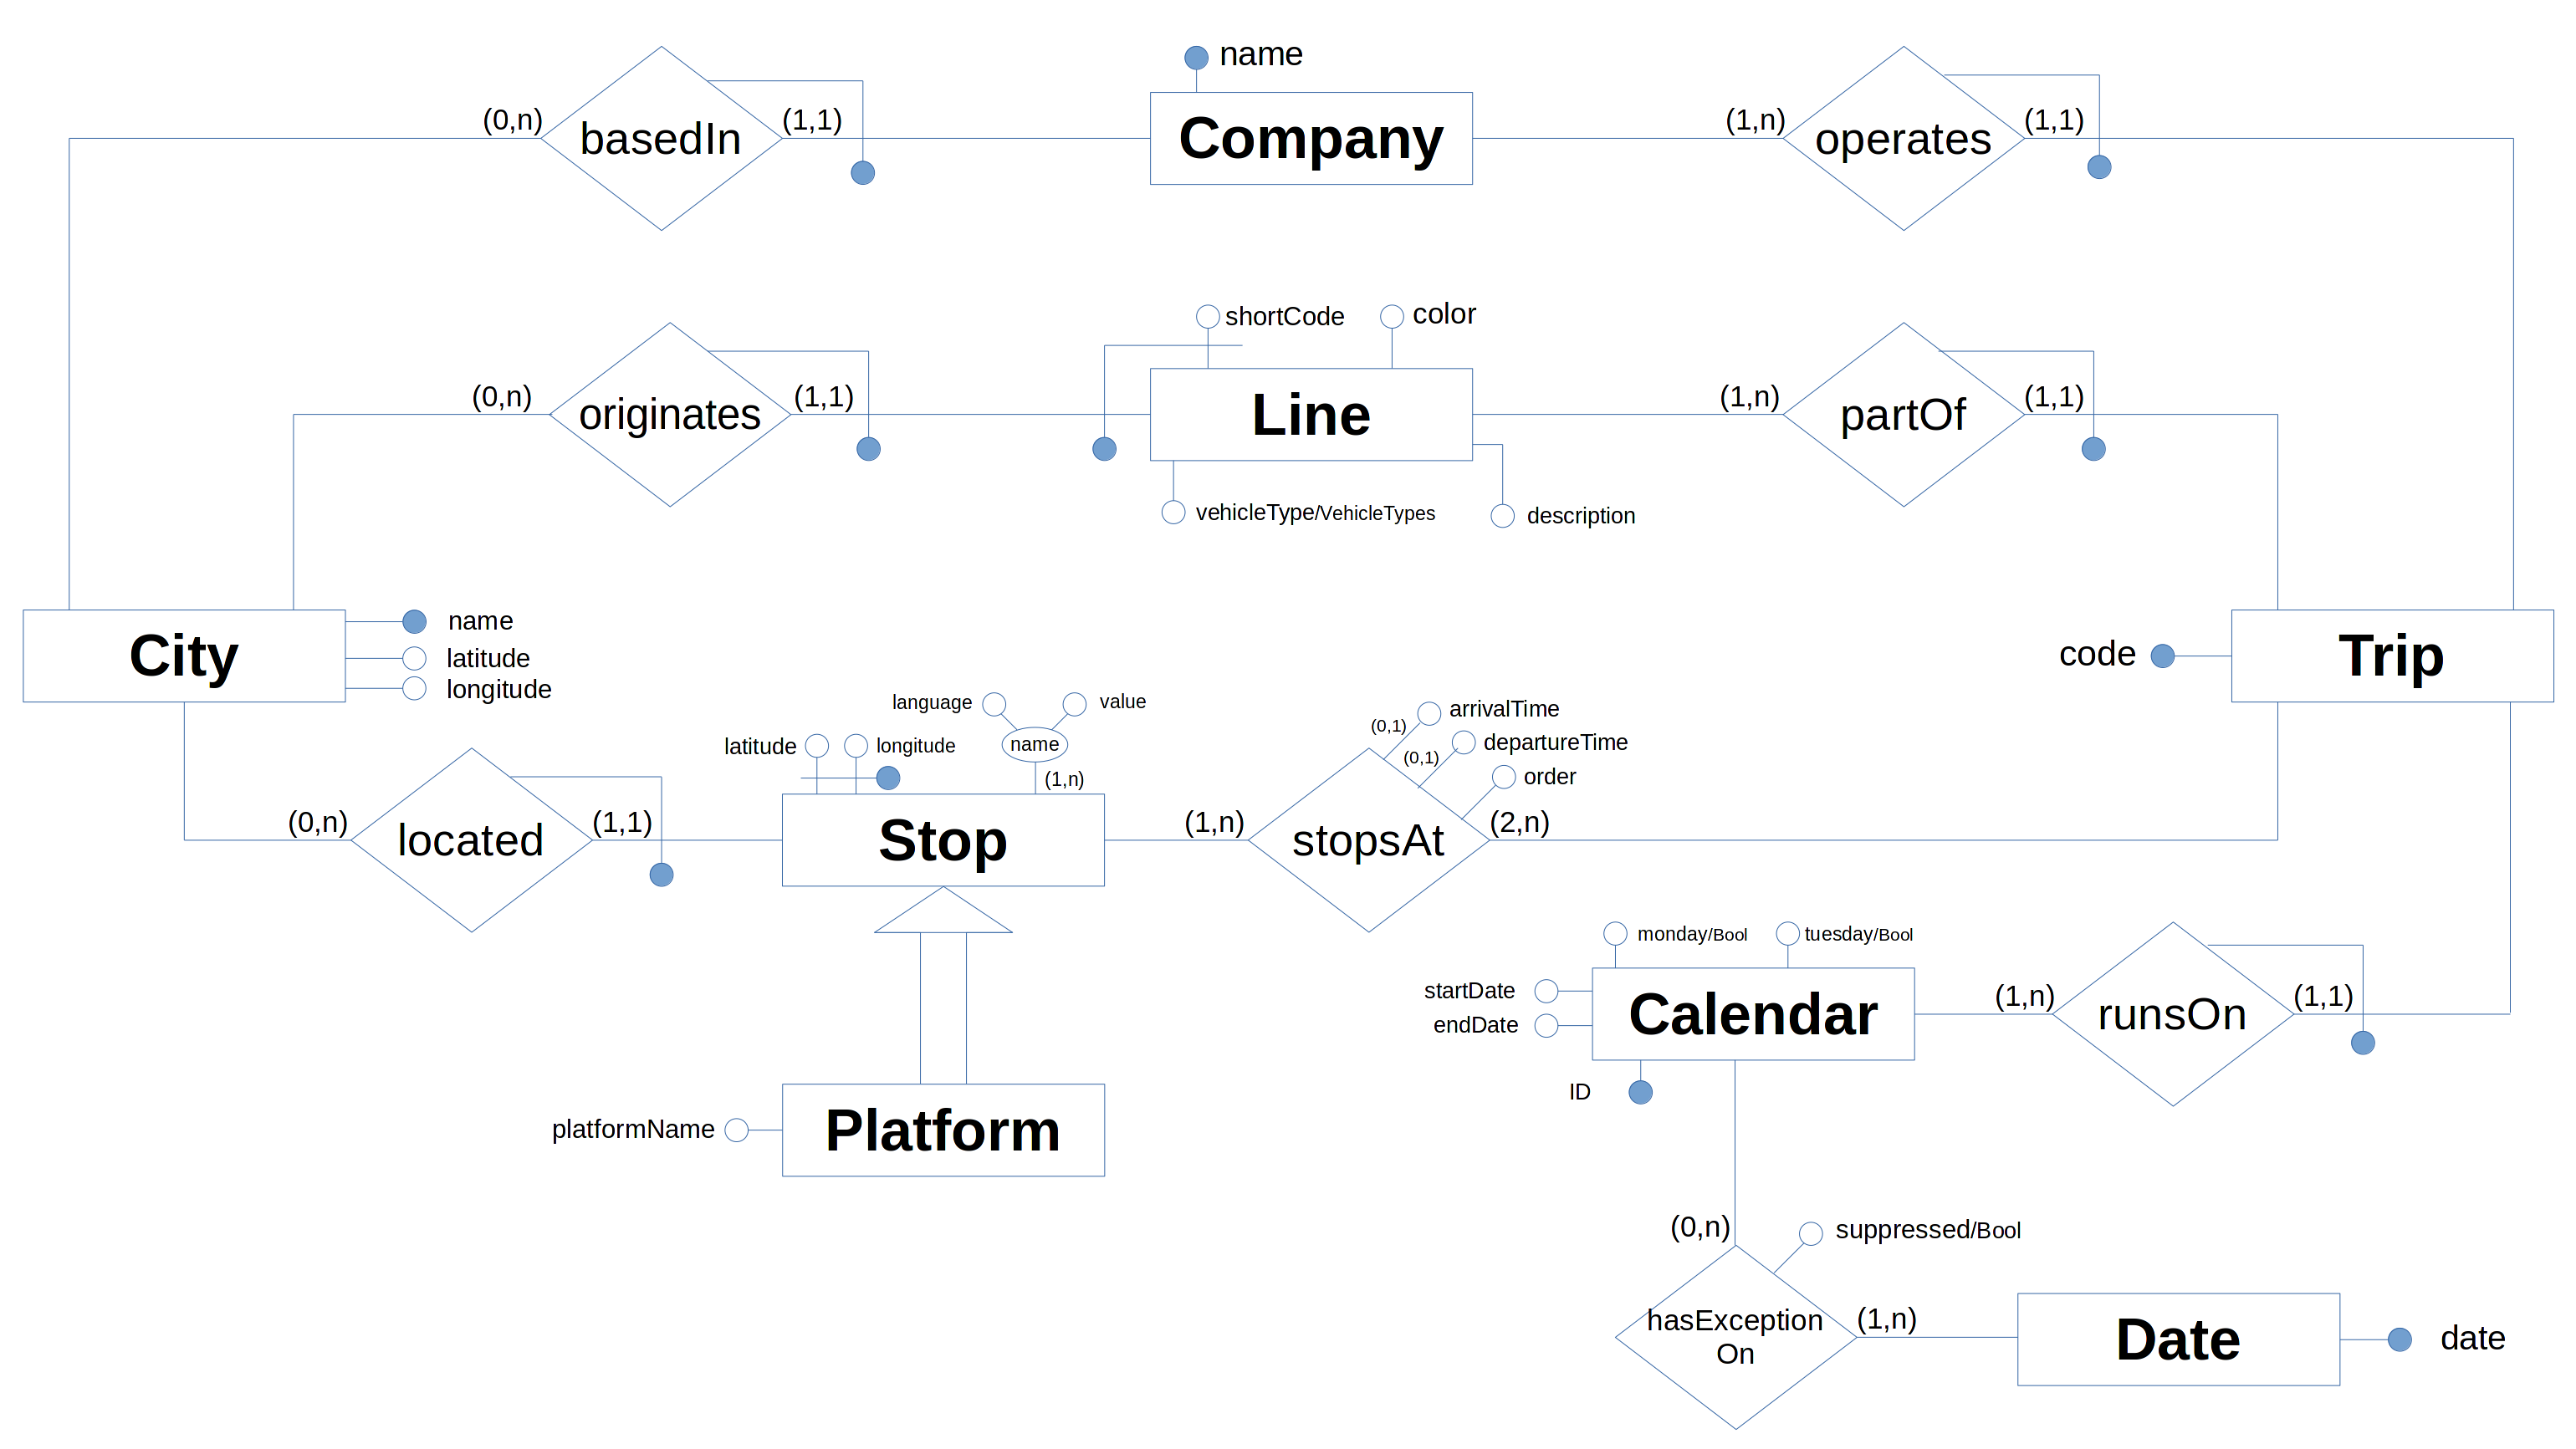
\includegraphics[height=\textheight]{imgs/diagram}
			\caption{ER Schema \\ {\footnotesize \textit{Note: not all attributes have been indicated in the schema. Please check the \hyperref[sec:dictionary]{data dictionary} for a complete overview}}}\label{img:diagram}
		\end{figure}
	\end{landscape}
	



\subsection{Glossary}

	\begin{table}[htb]
		\centering
		\begin{tabularx}{\columnwidth}{|c|C|}
			\hline
			\textbf{Term} & \textbf{Description} \\
			\hline
			\textbf{Stop} & Physical location in which passengers get on or off a vehicle  \\ \hline
			\textbf{Station} & Large stop consisting of many platform, where more than one vehicle can board passengers at the same time  \\ \hline
			\textbf{Platform} & Single stopping point inside a Station. It is represented by a number \\ \hline
			\textbf{Line} & Group of trips that follow the same route and is identified to the public with the same number or code  \\ \hline
			\textbf{Trip} & Ordered sequence of two or more stops, each with arrival and departure times \\ \hline
			\textbf{Calendar} & Defines when a trip runs in terms of date ranges and days of the week \\ \hline
			\textbf{Company} & Firm that is responsible of operating a trip \\
			\hline
		\end{tabularx}
		\caption{Glossary}\label{tbl:glossary}
	\end{table}

	\subsection{Data Dictionary}
	\label{sec:dictionary}

	\subsubsection{External Constraints}

	For completeness, all possible constraints have ben enlisted. Note that some of them can not be enforced at database level, either due to the lack functionalities of the DBMS or for the high complexity that they have. In particular, only constraints 1-4 will be checked by the DBMS.
	
	\begin{enumerate}
		\item For each tuple in the entity \texttt{Calendar}, the attribute \textit{endDate} must encode a date strictly greater than \textit{startDate}.
		
		\item For each tuple in the relationship \texttt{stopsAt}, the attribute \textit{departureTime} must encode a time greater or equal than \textit{arrivalTime}.
		
		\item In the relationship \texttt{stopsAt}, for the first stop of each \texttt{trip} (with \textit{order=1}), the attribute \textit{arrivalTime} must be omitted and \textit{departureTime} must be specified. For the last stop (with maximal \textit{order} for the trip), the attribute \textit{arrivalTime} must be specified and \textit{departureTime} must be omitted. For all the other stops, both attributes must be present.
		
		\item In the relationship \texttt{stopsAt}, the attribute \textit{order} must be equal to \texttt{1} for the first stop of a trip, and should be incremented by one for subsequent stops.
		
		\item In the relationship \texttt{stopsAt}, for every pair of tuples \textit{T1} and \textit{T2} within the same trip, if \textit{T1[order] < T2[order]}, then \textit{T1[departureTime] < T2[arrivalTime]}

		\item For a \texttt{Calendar}, the exceptional dates defined through the \texttt{hasExceptionOn} relationship must be in between \textit{startDate} and \textit{endDate}. Moreover, if \textit{suppressed=True} then the corresponding day of week has value \textit{True} (that is, trips will be exceptionally suppressed on that day, since normally on that day of week they do run). On the opposite, if \textit{suppressed=False} then the corresponding day of week has value \textit{False} (that is, trips will exceptionally run on that day, since normally they do not run on that day of week).
	\end{enumerate} 

	\subsubsection{Entities}
	
	See tables \ref{tbl:entites} and \ref{tbl:relationships}.
	
	\begin{table}[h!]
		\centering
		\begin{tabularx}{\columnwidth}{|c|C|C|c|}
			\hline
			\textbf{Entity} & \textbf{Description} & \textbf{Attributes} & \textbf{Identifiers} \\
			\hline
			\textbf{Calendar} & List of dates for which a trip runs. It defines a date range, with start and end date, together with the days of week in which the trip normally runs.
			
			Each day of week is a boolean value, so that if the value is \texttt{true} the trip runs on that day, otherwise it does not. & ID, startDate, endDate, monday, tuesday, wednesday, thursday, friday, saturday, sunday & \{ID\} \\ \hline
			\textbf{City} & Represents a city within the region of interest. & name, latitude, longitude & \{name\} \\ \hline
			\textbf{Company} & Transportation company responsible for running a set of trips & name & \{name\} \\ \hline
			\textbf{Date} & Specific date for which there is an exception (the corresponding trips are either suppressed or run exceptionally)& date & \{date\} \\ \hline
			\textbf{Line} & A public transportation line, ran by a specific kind of vehicle  & shortCode, description, color, vehicleType & \{shortCode, city\} \\ \hline
			\textbf{Stop} & Point in which a vehicle stops to allow passengers to board or get off & name, latitude, longitude & \{latitude, longitude\} \\ \hline
			\textbf{Platform} & Special kind of stop, represented by a code & platfornName & \{latitude, longitude\} \\ \hline
			\textbf{Trip} & Ordered sequence of two or more stops, each with arrival and departure times & code & \{code\} \\
			\hline
		\end{tabularx}
		\caption{Entities}\label{tbl:entites}
	\end{table}
	
	\subsubsection{Relationships}
	
	\begin{table}[h!]
		\centering
		\begin{tabularx}{\columnwidth}{|c|C|c|C|c|}
			\hline
			\textbf{Relationship} & \textbf{Description} & \textbf{Components} & \textbf{Attributes} & \textbf{Identifiers} \\
			\hline
			\textbf{basedIn} & Headquarter city of a company & City, Company & - & \{company\} \\ \hline
			\textbf{hasExceptionOn} & Exception for a date in the corresponding calendar & Date, Calendar & suppressed \textit{(true=suppressed, false=exceptional)} & \{date, calendar\} \\ \hline
			\textbf{located} & City where a stop is located & Stop, City & - & \{stop\} \\ \hline
			\textbf{operates} & Which company operates a specific trip & Company, Trip & - & \{trip\} \\ \hline
			\textbf{originates} & City from where a line departs & City, Line & - & \{line\} \\ \hline
			\textbf{partOf} & A trip is part of a line & Trip, Line & - & \{trip\} \\ \hline
			\textbf{runsOn} & Days of week in which the trip normally runs & Trip, Calendar & - & \{trip\} \\ \hline
			\textbf{stopsAt} & Stops traversed by a Trip, with time and order & Trip, Stop & arrivalTime, departureTime, order & \{trip, stop\} \\
			\hline
		\end{tabularx}
		\caption{Relationships}\label{tbl:relationships}
	\end{table}

\newpage
\subsection{Application Load}

	The indications of volume and frequency of operations are a rough estimation of a possible database instance in a small-sized region. The following assumptions were taken: \label{sec:assumptions}
	\begin{enumerate}[topsep=3pt,itemsep=0pt]
		\item On average, each calendar has 15 exceptional days;
		\item On average, each trip has nine stops;
		\item On average, 15 trips halt at any stop in the database every day;
		\item The stop names are fully translated in two languages. In general, it is assumed that there can be only \textit{full} translations (i.e. all tuples are translated in all defined languages);
		\item The timetable changes two times per year.
	\end{enumerate}

	\subsubsection{Table of Volumes}
	
	See table \ref{tbl:volumes}.
	
	\begin{table}[h]
		\centering
		\begin{tabular}{|c|c|c|}
			\hline
			\textbf{Concept} & \textbf{Construct} & \textbf{Volume} \\
			\hline
			City & Entity & 30 \\ \hline
			Stop & Entity & 75 \\ \hline
			Platform & Entity & 20 \\ \hline
			Trip & Entity & 500 \\ \hline
			Company & Entity & 5 \\ \hline
			Line & Entity & 25 \\ \hline
			Calendar & Entity & 10 \\ \hline
			Date & Entity & 200 \\ \hline
			basedIn & Relationship & 5 \\ \hline
			operates & Relationship & 500 \\ \hline
			originates & Relationship & 25 \\ \hline
			partOf & Relationship & 500 \\ \hline
			located & Relationship & 75 \\ \hline
			stopsAt & Relationship & 4500 \\ \hline
			runsOn & Relationship & 500 \\ \hline
			hasExceptionOn & Relationship & 150 \\ \hline
		\end{tabular}
		\caption{Table of Volumes}\label{tbl:volumes}
	\end{table}

	\newpage
	\subsubsection{List of Operations}
	
	\begin{enumerate}[itemsep=1.5pt]
		\item Get a list of \textit{(maximum)} ten stops with name in a specific language matching the user-given string;
		\item Get a list of \textit{(maximum)} ten stops with name in a specific language that are contained in a set of coordinates;
		\item Find the next ten trips, with line and company information, that depart from a specific stop at a given date and time \textit{(assuming that the stop coordinates are known)};
		\item Find the next ten trips departing from one stop and arriving at another one, at a given date and time \textit{(assuming that the stop coordinates are known)};
		\item Add a new company given the name and the headquarter city, \textit{and considering that all possible cities are already loaded into the database};
		\item Add a new line given short code, color, type of vehicle and city, \textit{and considering that all possible cities are already loaded into the database};
		\item Add a new trip given the code, the timetable, the operating company and the calendar;
		\item Modify the schedule for a calendar knowing its code (add one exceptional date)
	\end{enumerate}

	\begin{table}[h!]
		\centering
		\begin{tabular}{|c|c|c|}
			\hline
			\textbf{Op.} & \textbf{Type} & \textbf{Frequency} \\
			\hline
			1 & interactive & 500 / day \\ \hline
			2 & interactive & 200 / day \\ \hline
			3 & interactive & 500 / day \\ \hline
			4 & interactive & 750 / day \\ \hline
			5 & batch & 5 / year \\ \hline
			6 & batch & 25 / year \\ \hline
			7 & batch & 500 / year \\ \hline
			8 & batch & 500 / year \\ \hline
		\end{tabular}
		\caption{Frequency of operations}\label{tbl:operations}
	\end{table}
